  \subsection{Medición de factor de potencia en un circuito con control de ángulo de conducción}

Para el siguiente experimento se emplea el mismo circuito de la sección anterior. 
Ésta vez se conecta al medidor digital para medir 
el factor de potencia.

\begin{figure}[H]
  \centering
  \frame{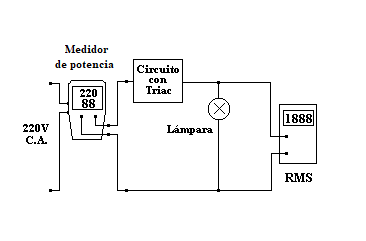
\includegraphics[width=0.5 \textwidth]{Imagenes/ActividadPractica/MedicionDeFactorDePotenciaConCircuitoTriac/Circuito_Medicion_FP_TriacDiac.png}}
  \caption{Circuito de medición de factor de potencia.}
  \label{fig:CircuitoMideFDP}
\end{figure}

Una vez realizada la conexión, se debe variar el potenciómetro del circuito 
de control de disparo, hasta lograr que la tensión eficaz de 
salida sea de 110~V.

\begin{figure}[H]
  \centering
  \frame{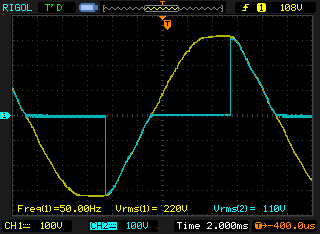
\includegraphics[width=0.5 \textwidth]{Imagenes/ActividadPractica/MedicionDeFactorDePotenciaConCircuitoTriac/Exp3_AnguloDisparoPara110Vrms.png}}
  \caption{Forma de onda para una tensión eficaz de 110[V].}
  \label{fig:SeñalExp3}
\end{figure}

 En éste punto se mide el factor de potencia inicial, 
 cuyo valor es de 0,47.

 \begin{figure}[H]
  \centering
  \frame{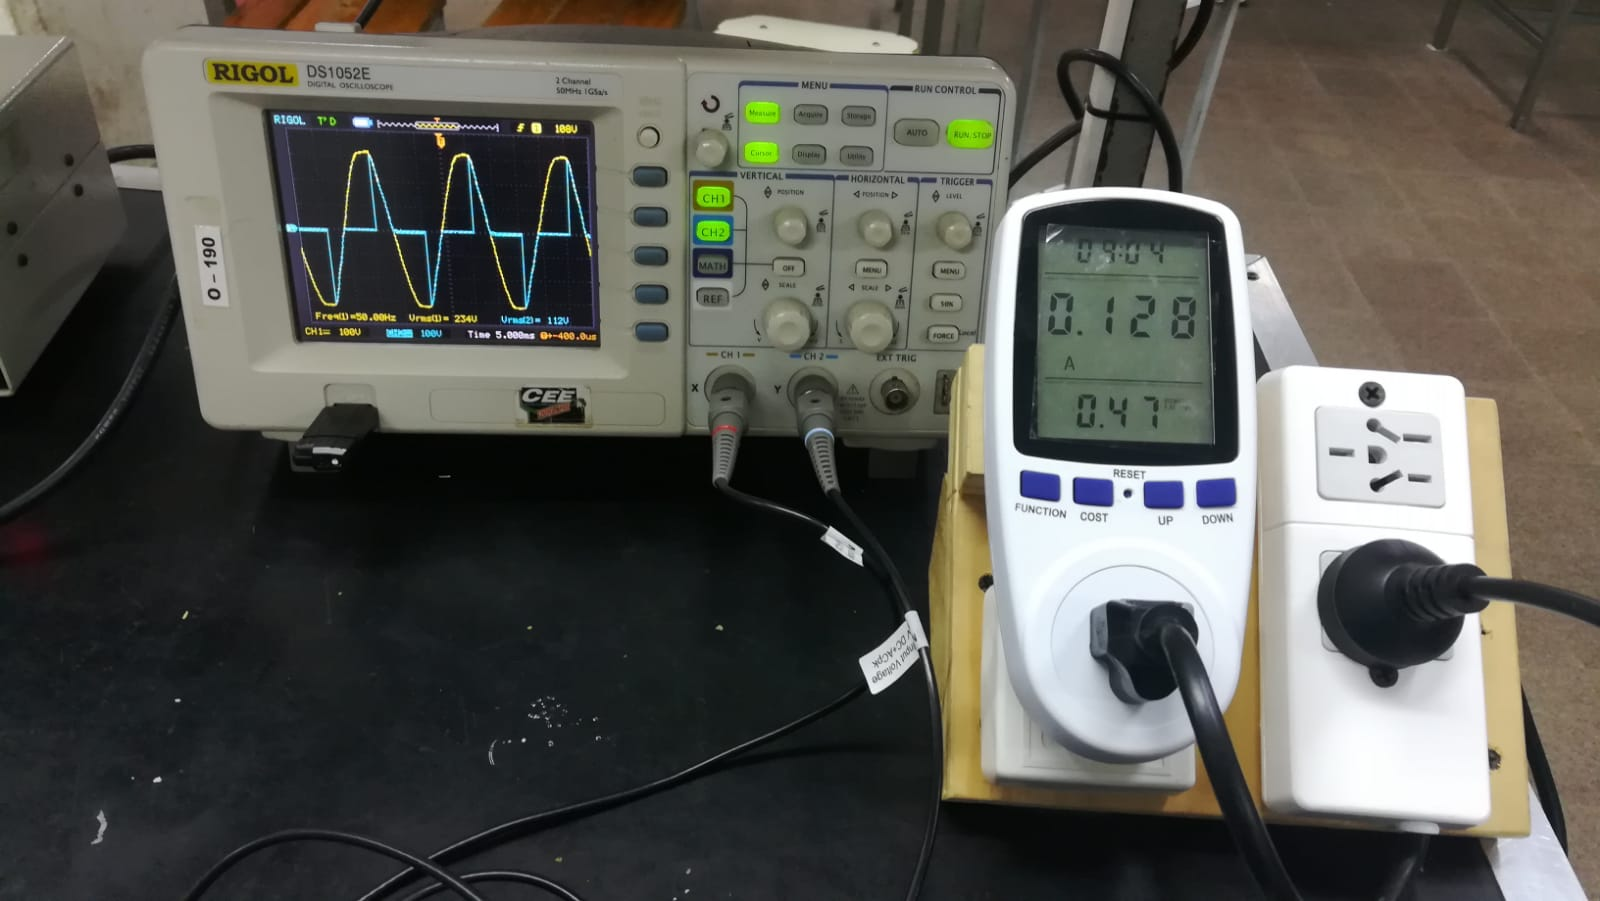
\includegraphics[width=0.5 \textwidth]{Imagenes/ActividadPractica/MedicionDeFactorDePotenciaConCircuitoTriac/Exp3_FDPcon110Vrms.jpeg}}
  \caption{Factor de potencia inicial.}
  \label{fig:FDPExp3}
\end{figure}

Al conectar el capacitor de corrección, se observa que el factor 
de potencia aumenta a 0,55, como muestra la Figura~\ref{fig:FDPCorregidoExp3}. 
Ésto indica que la carga total del circuito en conjunto, se comporta de manera inductiva.

 \begin{figure}[H]
  \centering
  \frame{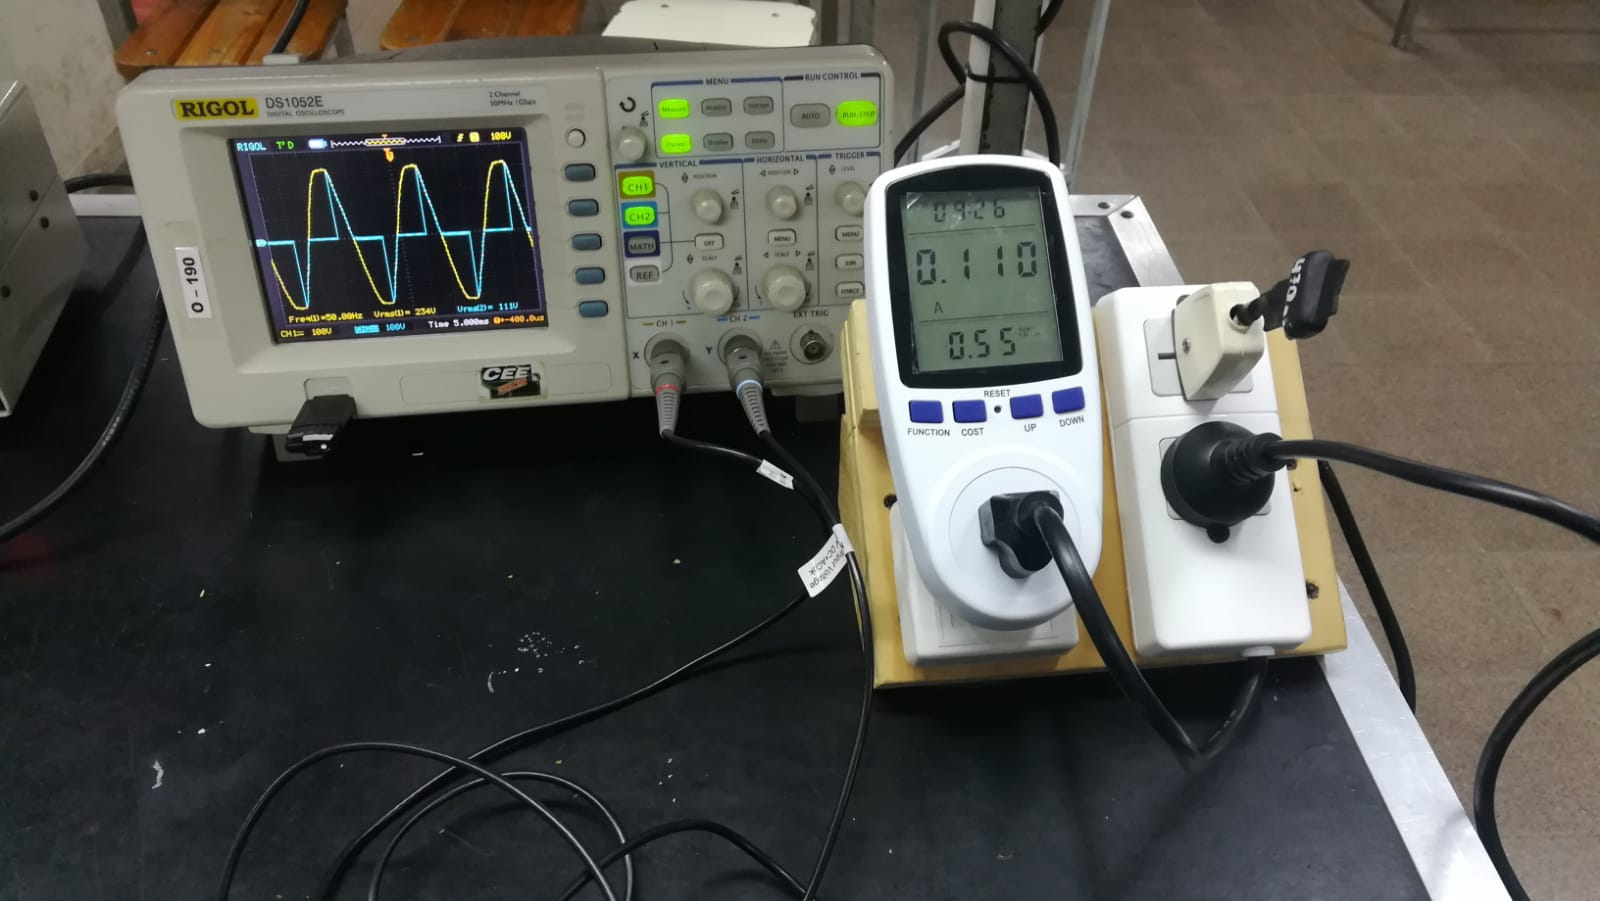
\includegraphics[width=0.5 \textwidth]{Imagenes/ActividadPractica/MedicionDeFactorDePotenciaConCircuitoTriac/Exp3_FDPConCapacitor.jpeg}}
  \caption{Factor de potencia corregido.}
  \label{fig:FDPCorregidoExp3}
\end{figure}
